% ---
% Arquivo com os anexos do Trabalho de Conclusão de Curso dos alunos
% Gabriel Takaoka Nishimura, Felippe Demarqui Ramos e Vivian Kimie Isuyama 
% da Escola Politécnica da Universidade de São Paulo
% ---
\chapter{Diagramas da Arquitetura}

\begin{figure}[!htb]
	\caption{\label{fig_sindrome_arq}Arquitetura do módulo de cálculo das síndromes.}
	\centering%%trim={<left> <lower> <right> <upper>}
	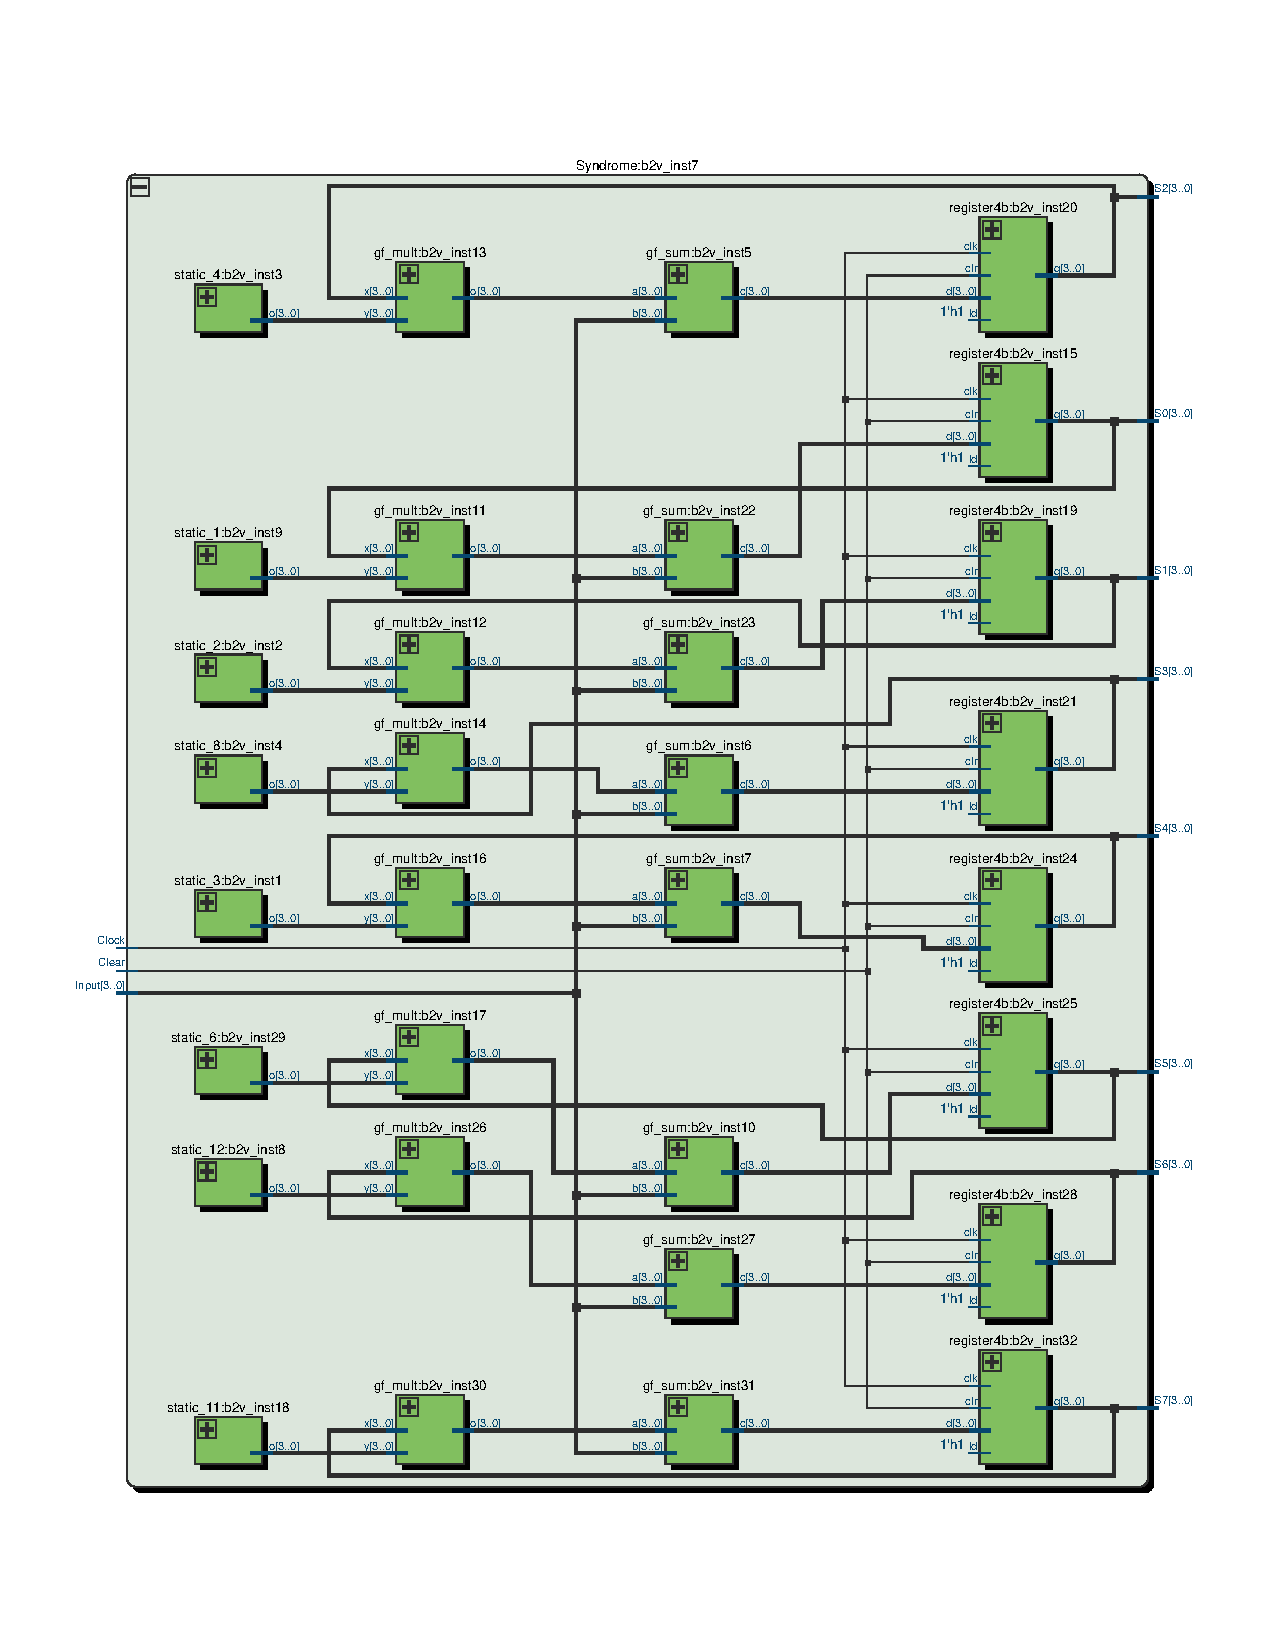
\includegraphics[width=1\textwidth, trim={2cm 5cm 2cm 5cm}]{RS/SindromeRTL.pdf}
	\legend{}
\end{figure}

\begin{figure}[!htb]
	\caption{\label{fig_berlekamp_arq}Arquitetura do módulo de Berlekamp-Massey.}
	\centering
	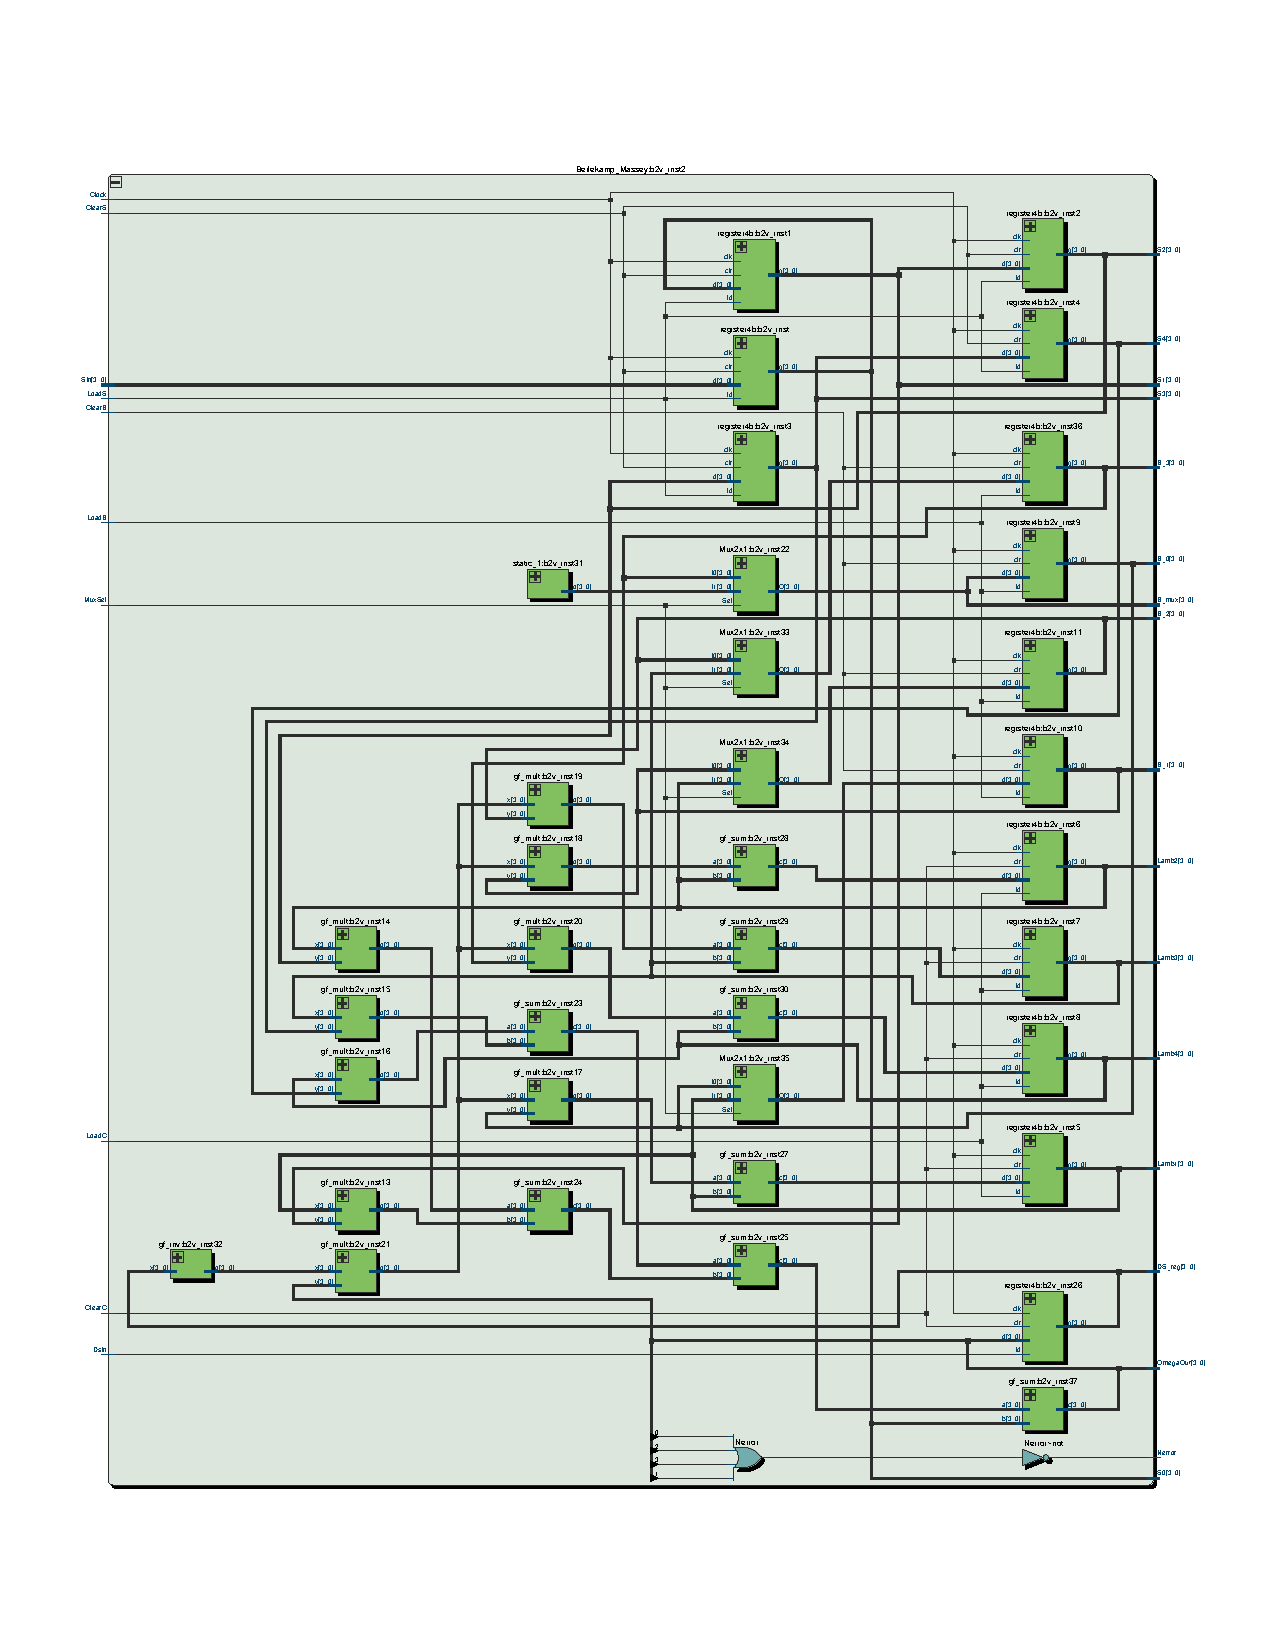
\includegraphics[width=1\textwidth, trim={2cm 5cm 2cm 5cm}]{RS/BerlekampRTL.pdf}
	\legend{}
\end{figure}

\begin{figure}[!htb]
	\caption{\label{fig_chienloc_arq}Arquitetura do módulo de busca de Chien: localização de erros.}
	\centering%%trim={<left> <lower> <right> <upper>}
	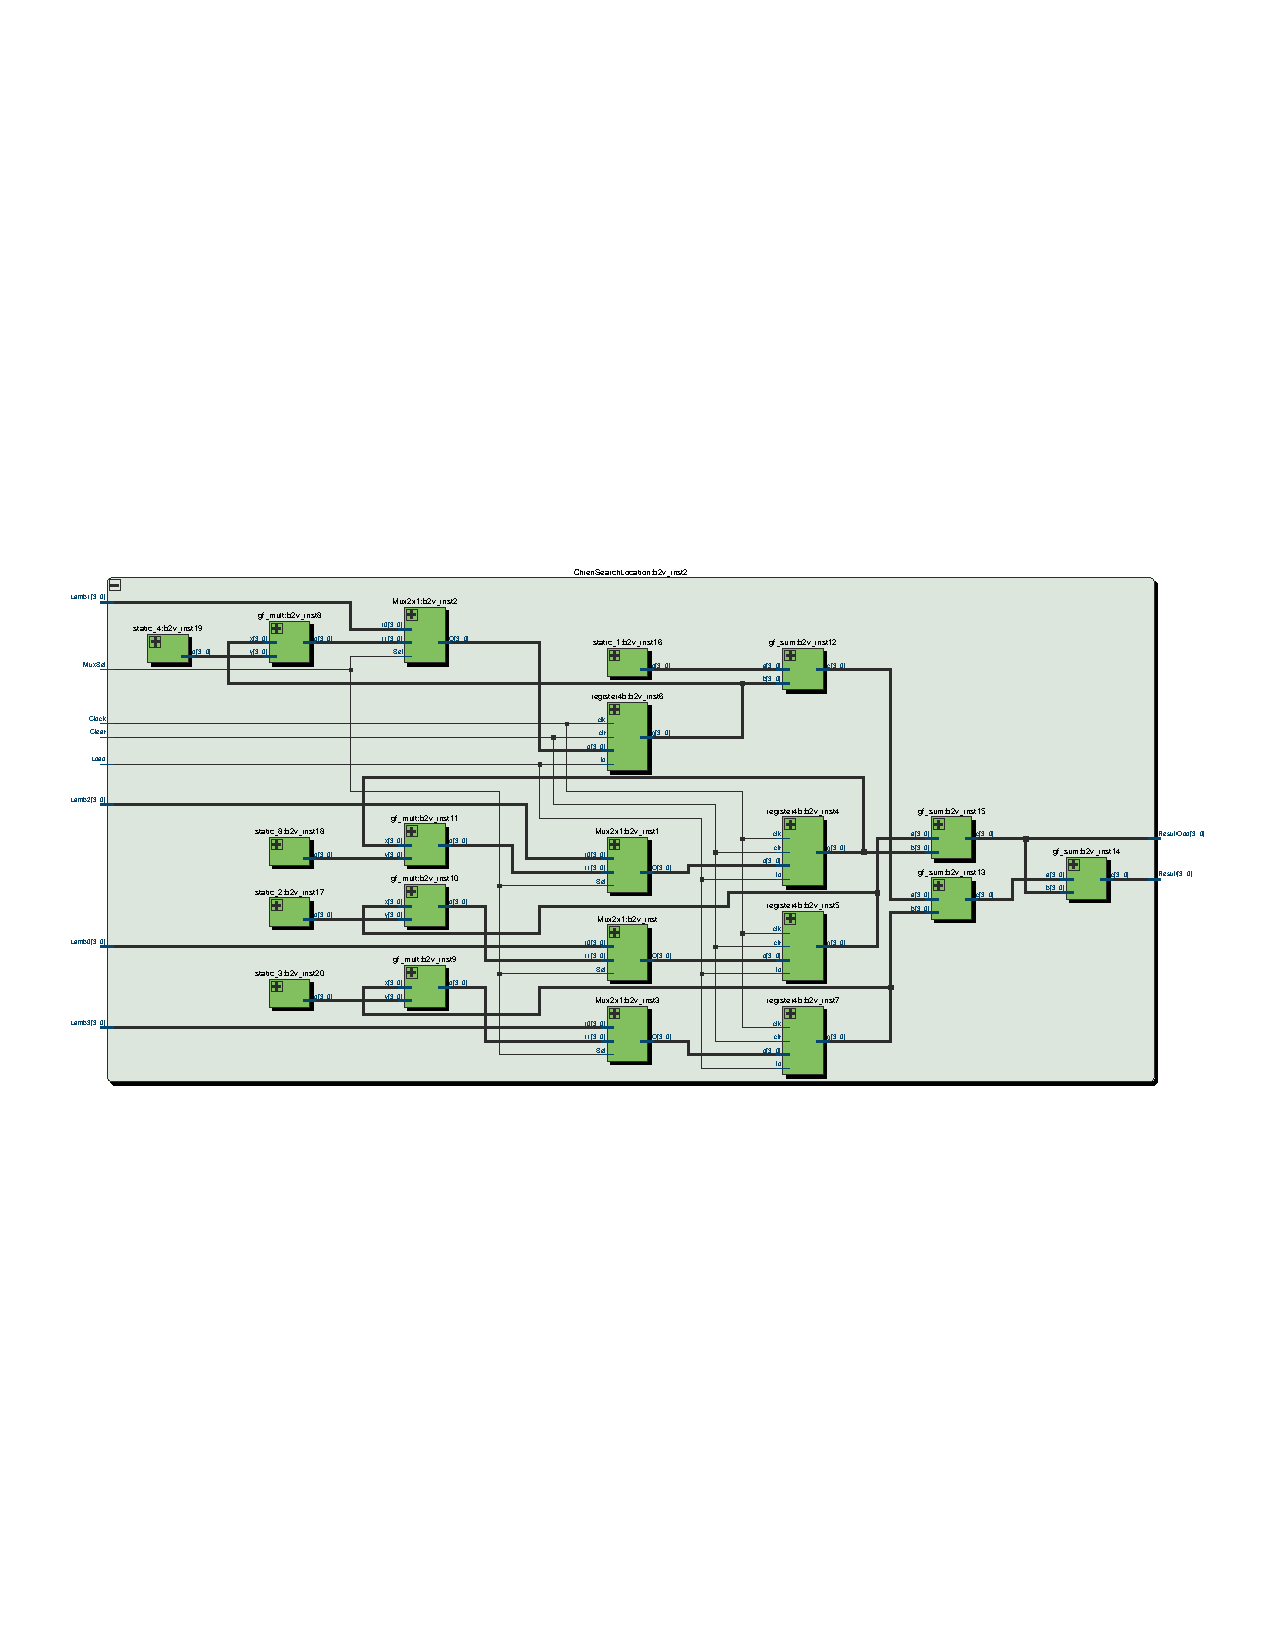
\includegraphics[width=1\textwidth, trim = {2cm 7cm 2cm 7cm}]{RS/ChienLocationRTL.pdf}
	\legend{}
\end{figure}

\begin{figure}[!htb]
	\caption{\label{fig_chienval_arq}Arquitetura do módulo de busca de Chien: valores de erros.}
	\centering %%trim={<left> <lower> <right> <upper>}
	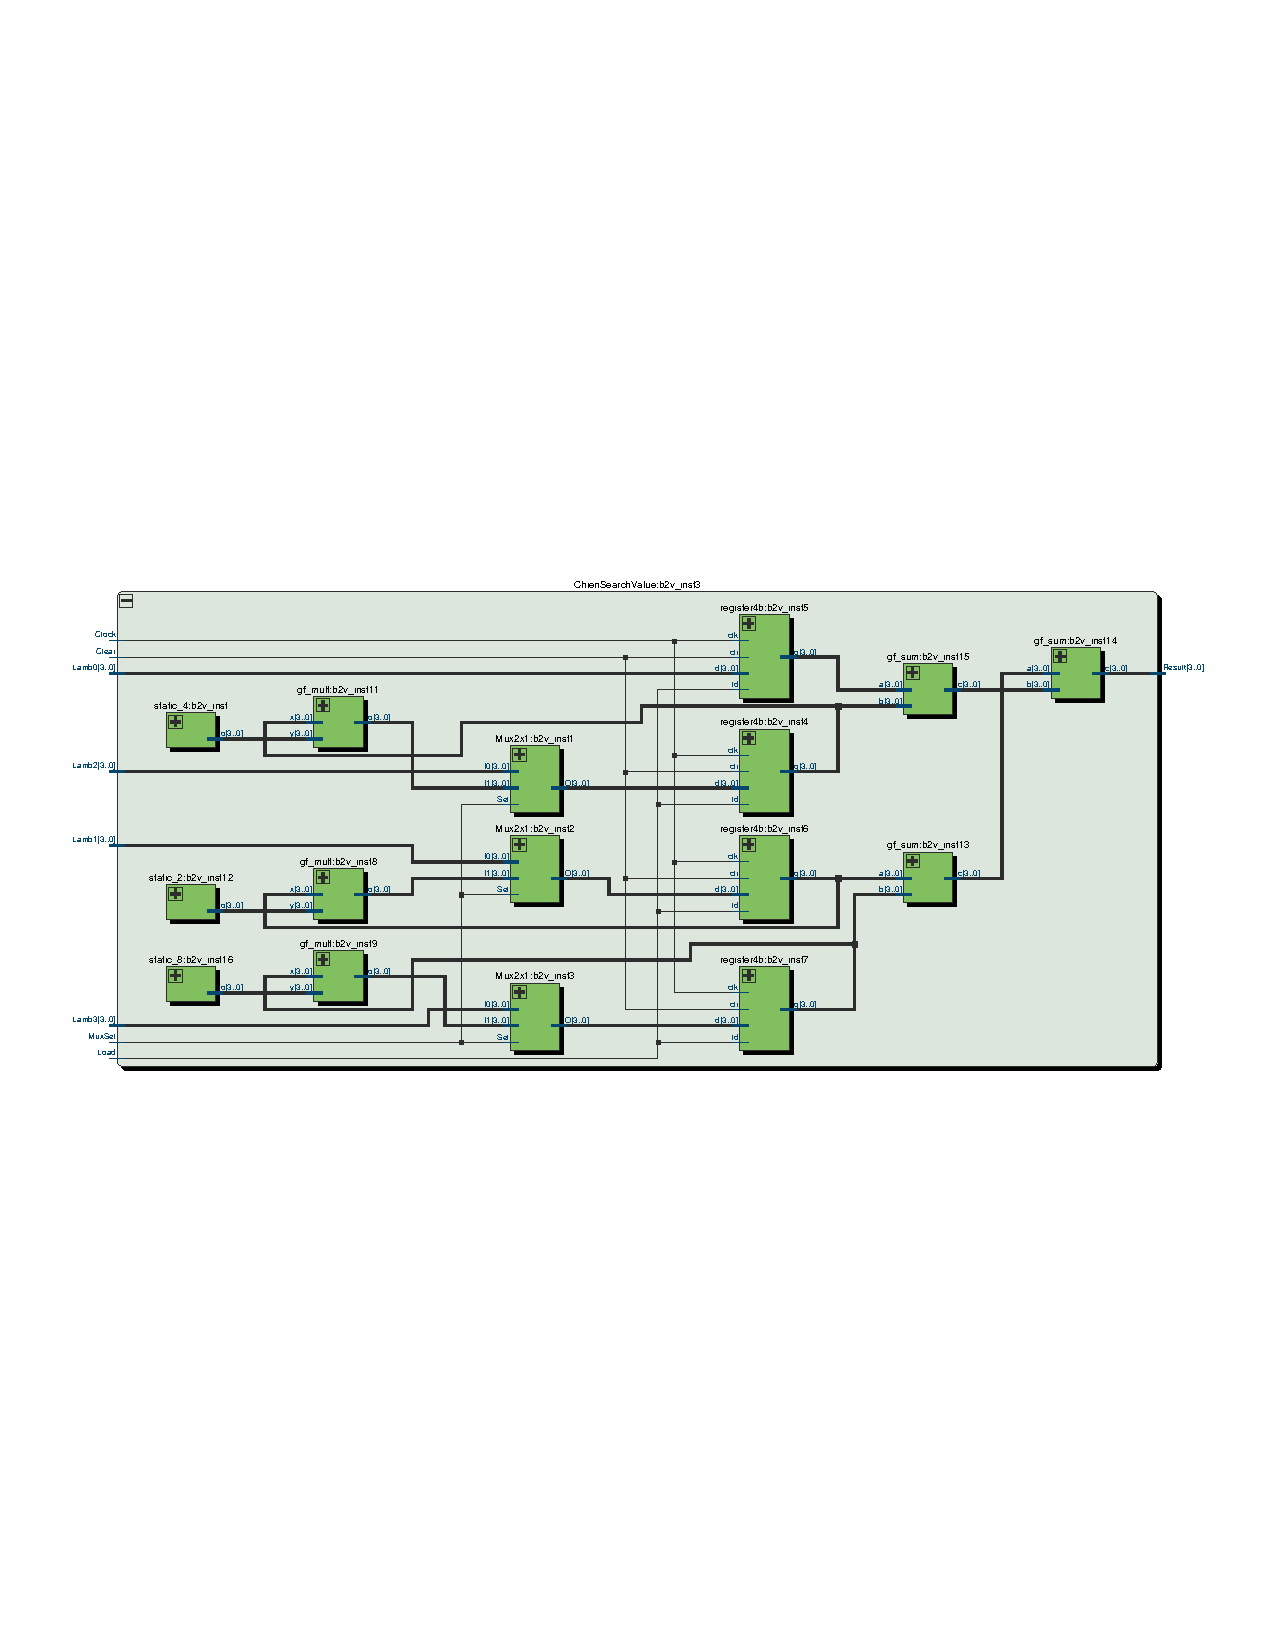
\includegraphics[width=1\textwidth,  trim = {2cm 7cm 2cm 7cm}]{RS/ChienValueRTL.pdf}
	\legend{}
\end{figure}